\documentclass{beamer}
\usepackage[english, russian]{babel}
\usepackage[T2A]{fontenc}
\usepackage[utf8]{inputenc}
\usepackage{indentfirst}
\usepackage{amsmath, amsfonts, amssymb, amsthm, mathtools}
\usepackage[export]{adjustbox}
\usepackage{graphicx} 
\graphicspath{ {./images/} }

\usepackage{subcaption}
\usepackage{verbatim}

\usepackage{minted}{\setlength{\parskip}{0pt}}

\usepackage{hyperref}

\hypersetup{
    colorlinks=true,
    linkcolor=blue,
    filecolor=magenta,      
    urlcolor=black,
    pdftitle={Overleaf Example},
    pdfpagemode=FullScreen,
    }


\title{Отчет по лабораторной работе № 6. \\ Установка и настройка системы управления базами данных MariaDB} 
\author{Данила Стариков \\ НПИбд-02-22}
\date{2024}

\begin{document}

\maketitle
\newpage

\tableofcontents

\newpage
\section{Цель работы}
Приобретение практических навыков по установке и конфигурированию системы управления базами данных на примере программного обеспечения MariaDB. \newpage
\section{Выполнение работы}
\subsection{Установка MariaDB}
\begin{enumerate}
\item Загрузили операционную систему и перешли в рабочий каталог с проектом:
  \begin{minted}{bash}
    cd /var/tmp/dastarikov/vagrant
  \end{minted}

\item Запустили виртуальную машину \texttt{server}:
  \begin{minted}{bash}
    make server-up
  \end{minted}

\item На виртуальной машине server вошли под своим пользователем и открыли терминал. Перешли в режим суперпользователя:
\begin{minted}{bash}
  sudo -i
\end{minted}
\item Установили необходимые для работы с базами данных пакеты:
  \begin{minted}{bash}
    dnf -y install mariadb mariadb-server
  \end{minted}
\item Просмотрели конфигурационные файлы \texttt{mariadb} в каталоге \texttt{/etc/my.cnf.d} и в файле \texttt{/etc/my.cnf}.
\item Для запуска и включения программного обеспечения \texttt{mariadb} использовали (Рис. \ref{01}):
  \begin{minted}{bash}
    systemctl start mariadb
    systemctl enable mariadb
  \end{minted}

\begin{center}
    \centering
    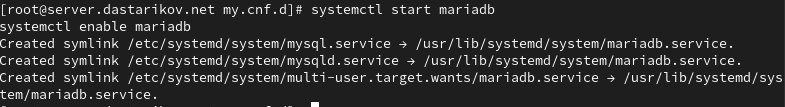
\includegraphics[width=\textwidth]{../images/image01.png}
    \captionof{figure}{Запуск ПО \texttt{mariadb}.}
    \label{01}
\end{center}

\item Убедились, что \texttt{mariadb} прослушивает порт (Рис. \ref{02}), используя 
  \begin{minted}{bash}
    ss -tulpen | grep mysql
  \end{minted}

\begin{center}
    \centering
    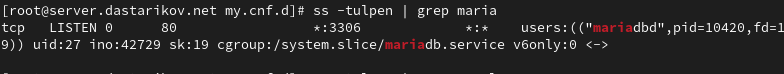
\includegraphics[width=\textwidth]{../images/image02.png}
    \captionof{figure}{Проверка прослушивания порта.}
    \label{02}
\end{center}

\item Запустили скрипт конфигурации безопасности \texttt{mariadb}, используя:
  \begin{minted}{bash}
    mysql_secure_installation
  \end{minted}
С помощью запустившегося диалога и путём выбора [Y/n] установили пароль для пользователя \texttt{root} базы данных, отключили удалённый корневой доступ и удалили тестовую базу данных и любых анонимных пользователей (Рис. \ref{03}).

\begin{center}
    \centering
    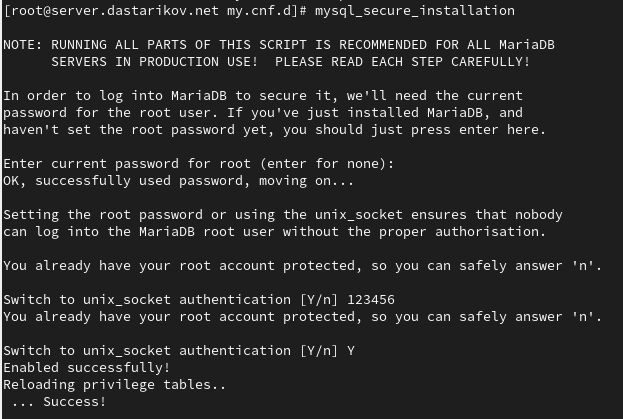
\includegraphics[width=\textwidth]{../images/image03.png}
    \captionof{figure}{Настройка конфигурации безопасности \texttt{mariadb}.}
    \label{03}
\end{center}

\item Для входа в базу данных с правами администратора базы данных ввели (Рис. \ref{04})
  \begin{minted}{bash}
    mysql -u root -p
  \end{minted}

\begin{center}
    \centering
    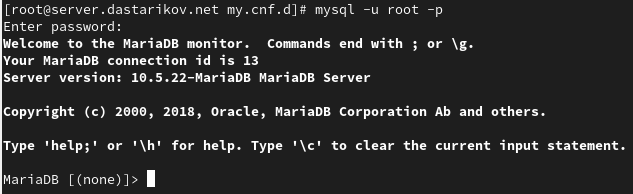
\includegraphics[width=\textwidth]{../images/image04.png}
    \captionof{figure}{Вход в базу данных с правами администратора.}
    \label{04}
\end{center}

\item Просмотрели список команд MySQL, введя \texttt{\textbackslash h} (Рис. \ref{05}).

\begin{center}
    \centering
    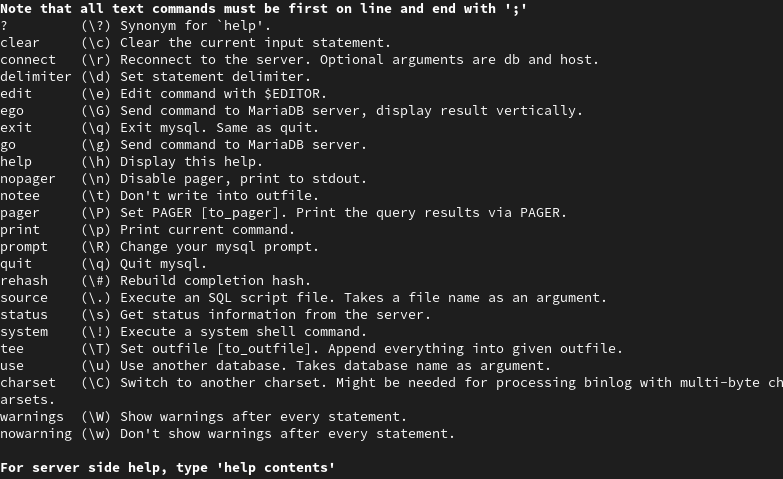
\includegraphics[width=\textwidth]{../images/image05.png}
    \captionof{figure}{Просмотр списка команд MySQL.}
    \label{05}
\end{center}

\item Из приглашения интерактивной оболочки MariaDB для отображения доступных в настоящее время баз данных ввели MySQL-запрос (Рис. \ref{06})
\begin{minted}{sql}
  SHOW DATABASES;
\end{minted}

\begin{center}
    \centering
    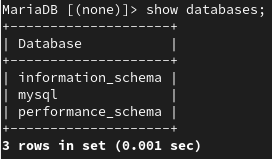
\includegraphics[width=\textwidth]{../images/image06.png}
    \captionof{figure}{Просмотр доступных баз данных.}
    \label{06}
\end{center}

Доступно три базы данных: \texttt{information\_schema}, \texttt{mysql}, \texttt{perfomance\_schema}.

\item Для выхода из интерфейса интерактивной оболочки MariaDB ввели (Рис. \ref{07})
  \begin{minted}{sql}
    exit;
  \end{minted}
\end{enumerate}

\begin{center}
    \centering
    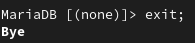
\includegraphics[width=\textwidth]{../images/image07.png}
    \captionof{figure}{Выход из интерактивной оболочки MariaDB.}
   \label{07}
\end{center}

\subsection{Конфигурация кодировки символов}
\begin{enumerate}
\item Вошли в базу данных с правами администратора:
  \begin{minted}{bash}
    mysql -u root -p
  \end{minted}
\item Для отображения статуса MariaDB ввели из приглашения интерактивной оболочки MariaDB (Рис. \ref{08}):
  \begin{minted}{sql}
    status
  \end{minted}

\begin{center}
    \centering
    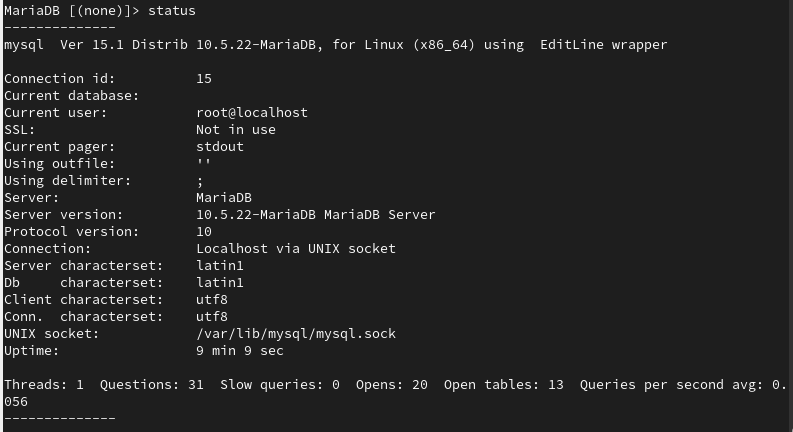
\includegraphics[width=\textwidth]{../images/image08.png}
    \captionof{figure}{Просмотр статуса MariaDB.}
    \label{08}
\end{center}

\item В каталоге \texttt{/etc/my.cnf.d} создали файл \texttt{utf8.cnf}:
  \begin{minted}{bash}
    cd /etc/my.cnf.d
    touch utf8.cnf
  \end{minted}
  Открыли его на редактирование и указали в нём следующую конфигурацию:
  \begin{minted}{bash}
    [client]
    default-character-set = utf8
    [mysqld]
    character-set-server = utf8
  \end{minted}
\item Перезапустили MariaDB:
  \begin{minted}{bash}
    systemctl restart mariadb
  \end{minted}
\item Вошли в базу данных с правами администратора и посмотрели статус MariaDB (Рис. \ref{10}).

\begin{center}
    \centering
    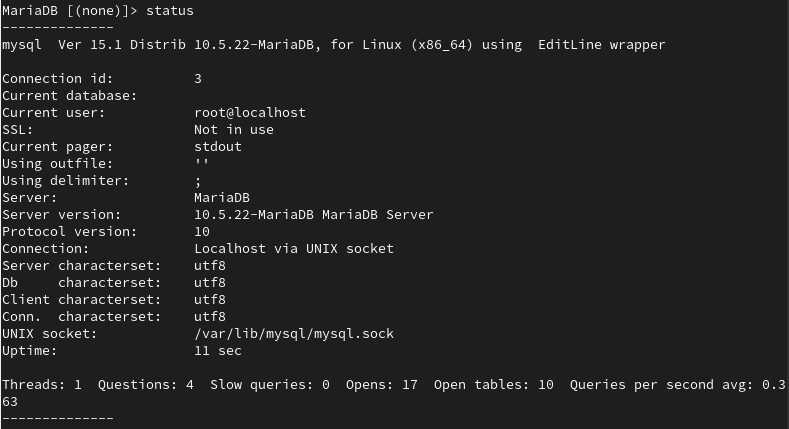
\includegraphics[width=\textwidth]{../images/image10.png}
    \captionof{figure}{Просмотр статуса MariaDB после изменения конфигурации.}
    \label{10}
\end{center}
Теперь в базах данных и в выводе запросов будет использоваться кодировка UTF-8.
\end{enumerate}
\subsection{Создание базы данных}
\begin{enumerate}
\item Вошли в базу данных с правами администратора (Рис. \ref{21}):
  \begin{minted}{bash}
    mysql -u root -p
  \end{minted}
\item Создали базу данных с именем \texttt{addressbook} (Рис. \ref{21}):
  \begin{minted}{sql}
    CREATE DATABASE addressbook CHARACTER SET utf8 COLLATE utf8_general_ci;
  \end{minted}
\item Перешли к базе данных \texttt{addressbook} (Рис. \ref{21})
  \begin{minted}{sql}
    USE addressbook;
  \end{minted}
\item Отобразили имеющиеся в базе данных \texttt{addressbook} таблицы (Рис. \ref{21}):
  \begin{minted}{sql}
    SHOW TABLES;
  \end{minted}

\begin{center}
    \centering
    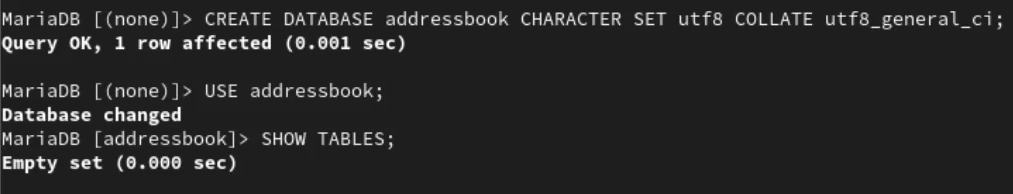
\includegraphics[width=\textwidth]{../images/image21.png}
    \captionof{figure}{Создание базы данных \texttt{addressbook}.}
    \label{21}
\end{center}

\item Создали таблицу \texttt{city} с полями \texttt{name} и \texttt{city} (Рис. \ref{11}):
  \begin{minted}{sql}
    CREATE TABLE city(name VARCHAR(40), city VARCHAR(40));
  \end{minted}

\item Заполнили несколько строк таблицы некоторыми данными по аналогии в соответствии с синтаксисом MySQL (Рис. \ref{11}):
  \begin{minted}{sql}
    INSERT INTO city(name,city) VALUES ('Иванов','Москва');
  \end{minted}
  В частности, добавили в базу сведения о Петрове и Сидорове (Рис. \ref{11}):

\begin{minted}{sql}
  INSERT INTO city(name,city) VALUES ('Петров','Сочи');
  INSERT INTO city(name,city) VALUES ('Сидоров','Дубна');
  \end{minted}

\begin{center}
    \centering
    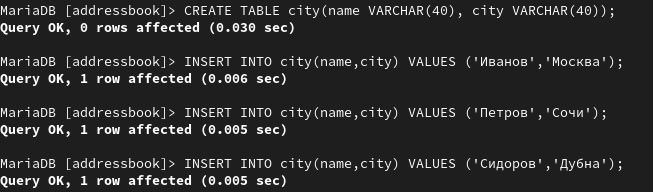
\includegraphics[width=\textwidth]{../images/image11.png}
    \captionof{figure}{Создание и заполнение таблицы.}
    \label{11}
\end{center}

\item Сделали следующий MySQL-запрос (Рис. \ref{12}):
  \begin{minted}{sql}
    SELECT * FROM city;
  \end{minted}

\begin{center}
    \centering
    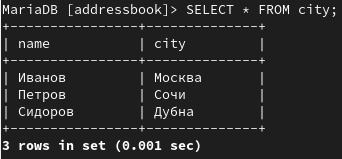
\includegraphics[width=\textwidth]{../images/image12.png}
    \captionof{figure}{Просмотр вхождений таблицы.}
    \label{12}
\end{center}

Запрос вывел все вхождения таблицы, которые былы добавлены.

\item Создали пользователя для работы с базой данных \texttt{addressbook} и задали для него пароль (Рис. \ref{13}):
  \begin{minted}{sql}
    CREATE USER dastarikov@'%' IDENTIFIED BY 'password';
  \end{minted}
\item Предоставили права доступа созданному пользователю \texttt{dastarikov} на действия с базой данных \texttt{addressbook} (просмотр, добавление, обновление, удаление данных) (Рис. \ref{13}):
  \begin{minted}{sql}
    GRANT SELECT,INSERT,UPDATE,DELETE ON addressbook.* TO dastarikov@'%';
  \end{minted}
Обновили привилегии (права доступа) базы данных \texttt{addressbook} (Рис. \ref{13}):
  \begin{minted}{sql}
    FLUSH PRIVILEGES;
  \end{minted}

\begin{center}
    \centering
    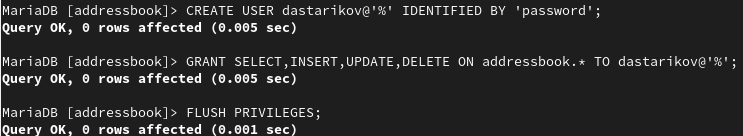
\includegraphics[width=\textwidth]{../images/image13.png}
    \captionof{figure}{Создание нового пользователя для работы с таблицей.}
    \label{13}
\end{center}

\item Посмотрели общую информацию о таблице \texttt{city} базы данных \texttt{addressbook} (Рис. \ref{14}):
  \begin{minted}{sql}
    DESCRIBE city;
  \end{minted}

\begin{center}
    \centering
    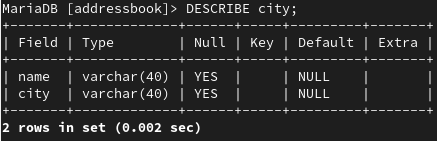
\includegraphics[width=\textwidth]{../images/image14.png}
    \captionof{figure}{Общая информация о таблице.}
    \label{14}
\end{center}

\item Вышли из окружения MariaDB:
  \begin{minted}{sql}
    quit
  \end{minted}
\item Просмотрели список баз данных (Рис. \ref{15}):
  \begin{minted}{bash}
    mysqlshow -u root -p
  \end{minted}

\begin{center}
    \centering
    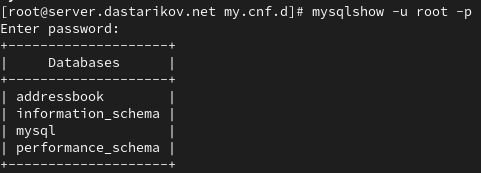
\includegraphics[width=\textwidth]{../images/image15.png}
    \captionof{figure}{Просмотр списка баз данных.}
    \label{15}
\end{center}

\item Просмотрели список таблиц базы данных \texttt{addressbook} (Рис. \ref{16}):
  \begin{minted}{bash}
    mysqlshow -u root -p addressbook
  \end{minted}
  или (Рис. \ref{17})
  \begin{minted}{bash}
    mysqlshow -u dastarikov -p addressbook
  \end{minted}

\begin{center}
    \centering
    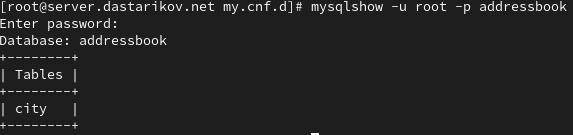
\includegraphics[width=\textwidth]{../images/image16.png}
    \captionof{figure}{Просмотр таблиц базы данных \texttt{addressbook} пользователем \texttt{root}.}
    \label{16}
\end{center}

\begin{center}
    \centering
    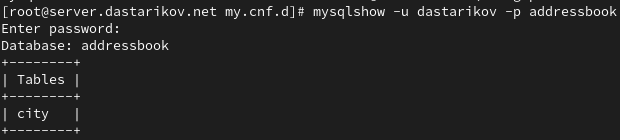
\includegraphics[width=\textwidth]{../images/image17.png}
    \captionof{figure}{Просмотр таблиц базы данных \texttt{addressbook} пользователем \texttt{dastarikov}.}
    \label{17}
\end{center}

\end{enumerate}
\subsection{Резервные копии}
\begin{enumerate}
\item На виртуальной машине \texttt{server} создали каталог для резервных копий (Рис. \ref{18}):
  \begin{minted}{bash}
    mkdir -p /var/backup
  \end{minted}
\item Сделали резервную копию базы данных \texttt{addressbook} (Рис. \ref{18}):
  \begin{minted}{bash}
    mysqldump -u root -p addressbook > /var/backup/addressbook.sql
  \end{minted}
\item Сделали сжатую резервную копию базы данных \texttt{addressbook} (Рис. \ref{18}):
  \begin{minted}{bash}
    mysqldump -u root -p addressbook | gzip > /var/backup/addressbook.sql.gz
  \end{minted}
\item Сделали сжатую резервную копию базы данных \texttt{addressbook} с указанием даты создания копии (Рис. \ref{18}):
  \begin{minted}{bash}
    mysqldump -u root -p addressbook | gzip >\$(date +/var/backup/addressbook.%Y%m%d.%H%M%S.sql.gz)
  \end{minted}
\item Восстановили базу данных \texttt{addressbook} из резервной копии (Рис. \ref{18}):
  \begin{minted}{bash}
    mysql -u root -p addressbook < /var/backup/addressbook.sql
  \end{minted}
\item Восстановили базу данных \texttt{addressbook} из сжатой резервной копии (Рис. \ref{18}):
  \begin{minted}{bash}
    zcat /var/backup/addressbook.sql.gz | mysql -u root -p addressbook
  \end{minted}
\end{enumerate}

\begin{center}
    \centering
    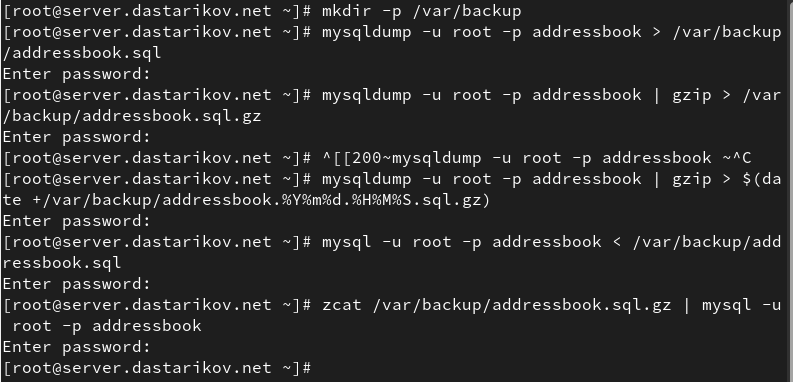
\includegraphics[width=\textwidth]{../images/image18.png}
    \captionof{figure}{Создание и восстановление резервной копии базы данных.}
    \label{18}
\end{center}

\subsection{Внесение изменений в настройки внутреннего окружения виртуальной машины}
\begin{enumerate}
\item На виртуальной машине server перешли в каталог для внесения изменений в настройки внутреннего окружения \texttt{/vagrant/provision/server}/, создали в нём каталог \texttt{mysql}, в который поместили в соответствующие подкаталоги конфигурационные файлы MariaDB и резервную копию базы данных addressbook (Рис. \ref{19}):
  \begin{minted}{bash}
    cd /vagrant/provision/server
    mkdir -p /vagrant/provision/server/mysql/etc/my.cnf.d
    mkdir -p /vagrant/provision/server/mysql/var/backup
    cp -R /etc/my.cnf.d/utf8.cnf /vagrant/provision/server/mysql/etc/my.cnf.d/
    cp -R /var/backup/* /vagrant/provision/server/mysql/var/backup/
  \end{minted}

\begin{center}
    \centering
    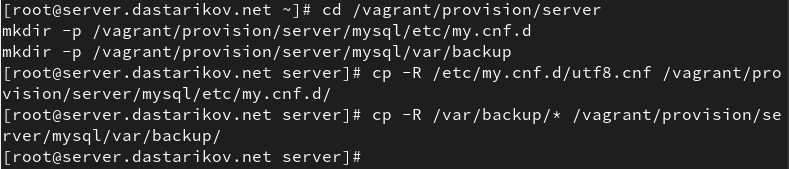
\includegraphics[width=\textwidth]{../images/image19.png}
    \captionof{figure}{Создание каталога для настроек внутреннего окружения.}
    \label{19}
\end{center}

\item В каталоге \texttt{/vagrant/provision/server} создали исполняемый файл \texttt{mysql.sh}:
  \begin{minted}{bash}
    cd /vagrant/provision/server
    touch mysql.sh
    chmod +x mysql.sh
  \end{minted}
  Открыв его на редактирование, прописали в нём следующий скрипт:
  \begin{minted}{bash}
    #!/bin/bash
    echo "Provisioning script $0"
    systemctl restart named
    echo "Install needed packages"
    dnf -y install mariadb mariadb-server
    echo "Copy configuration files"
    cp -R /vagrant/provision/server/mysql/etc/* /etc
    mkdir -p /var/backup
    cp -R /vagrant/provision/server/mysql/var/backup/* /var/backup
    echo "Start mysql service"
    systemctl enable mariadb
    systemctl start mariadb
    if [[ ! -d /var/lib/mysql/mysql ]]
    then
    echo "Securing mariadb"
    mysql_secure_installation <<EOF
    y
    123456
    123456
    y
    y
    y
    y
    EOF
    echo "Create database"
    mysql -u root -p123456 <<EOF
    CREATE DATABASE addressbook CHARACTER SET utf8 COLLATE utf8_general_ci;
    EOF
    mysql -u root -p123456 addressbook < /var/backup/addressbook.sql
    fi
  \end{minted}
  Этот скрипт, по сути, повторяет произведённые в работе действия по установке и настройке сервера баз данных.
\item Для отработки созданного скрипта во время загрузки виртуальных машин в конфигурационном файле Vagrantfile добавили в конфигурации сервера следующую запись:
  \begin{minted}{bash}
    server.vm.provision "server mysql",
    type: "shell",
    preserve_order: true,
    path: "provision/server/mysql.sh"
  \end{minted}
\end{enumerate}


\section{Выводы}
В результате выполнения лабораторной работы приобрели практические навыки по установке и конфигурированию системы управления базами данных на примере программного обеспечения MariaDB.
\end{document}
